%!TEX root = ../thesis.tex
% chapter 2

\chapter{Quasi-equilibrium phase coexisting supercritical fluid}
\label{sec:ch2}

Simple fluids are generally thought to assume a homogeneous phase in their supercritical state across all combinations of pressures and temperatures, although various response functions or transport properties may exhibit anomalous behavior, characterizing a state point as either more gas-like or liquid-like. While much research has been done in the past two decades on the intricacies of the supercritical phase in thermodynamic equilibrium, much fewer investigations have been done on out-of-equilibrium instances that may arise when working with fluids like carbon dioxide or argon. We examine regular compression-expansion cycles of an equal amount of argon pumped into a high-pressure chamber, crossing the critical pressure at twice the critical temperature. The fluid temporarily becomes sub-critical due to expansion cooling, and light scattering studies reveal the formation of sub-micron-sized droplets and nanometer-scale clusters, which are different from the spontaneous density fluctuations of supercritical background, and they last for a surprisingly long period \cite{lee2021quasi}. This phenomenon may be explained using a kinetic rate model of liquid droplet exchange with smaller clusters. Our findings suggest that supercritical fluids have non-equilibrium properties that may be relevant to their processing in industrial applications.



%----------------------------------------------------------------------------------------------------
\section{Inhomogeneity in supercritical phase}
\label{sec:ch2-1}

Supercritical fluids (SCFs), first observed in 1822 by Charles Cagniard de la Tour \cite{berche2009critical}, have fascinated scientific and industrial interest due to their unique properties, which include higher density than gas, lower viscosity than liquid, and intrinsically high-density fluctuations \cite{knez2014industrial, stauss2015review}. SCFs can enable enhanced chemical reaction speeds due to their reduced viscosity, better diffusivity, and superior solubility than liquid \cite{medina2012determination}. The selective extraction of molecules from natural materials \cite{sovova2012steps} and the synthesis of polymer nanocomposite foams \cite{lee2005polymer, matson1987rapid} are two uses of SCFs that have been intensively investigated. SCFs are employed as reaction mediums for chemical processes \cite{munshi2009supercritical} and in heat exchange systems \cite{duffey2005experimental}.


In contrast to subcritical fluids, which have discrete liquid and vapor phases, it is often assumed that SCFs have only one phase. Because they are homogeneous and structureless, SCFs have no surface tension or phase transition far from the critical point. However, over the last two decades, it has been discovered that as pressure, temperature, or density are varied across appropriate regions in the parameter space, SCFs can exhibit more liquid-like (LL) or gas-like (GL) properties \cite{simeoni2010widom, gorelli2006liquidlike, banuti2015crossing, maxim2019visualization, pipich2018densification, pipich2020polymorphic, prescher2017experimental, proctor2018liquid, bryk2017behavior}. These qualifications always refer to specific characteristics like sound dispersion \cite{simeoni2010widom, gorelli2006liquidlike}, unexpected variations in thermodynamic response functions \cite{banuti2015crossing}, or correlations in density fluctuations \cite{ploetz2019gas}, and always imply continuous variations of all relevant observables \cite{schienbein2018investigation}.

On the other hand, many industrial processes entail high non-equilibrium dynamics of SCFs, with large spatial and temporal rates of change. Meteorological flows in Venus's atmosphere, SCF extraction \cite{taylor1996supercritical}, and high-pressure flows in propulsion systems are all examples. Depending on the ambient pressure, the fluid fuel stream injected into an ambient fluid exhibits a combination of continuous thermodynamic and transport characteristics and discrete creation of ligaments and droplets modifications (Chap.10 in \cite{bellan2020high}). The fuel stream may form a fractal-like boundary in the intermediate (transcritical) pressure domain, blurring the distinction between two-phase and one-phase \cite{harstad2000all}.

These applications show that studying an SCF's transitory behavior in intense non-equilibrium situations with rapid disruptions may necessitate a more comprehensive investigation. We use argon as an archetypal inert gas to perform controlled compression-expansion cycles. Light scattering tests show that liquid sub-micron-sized droplets and nanometer-scale clusters occur following initial fast expansion and cooldown under subcritical circumstances. These float in the chamber and last a remarkable amount of time as metastable liquid-like (LL) compact fluid bundles before being absorbed into the gas-like supercritical background \cite{harstad2000all}. The LL droplets' lifetime falls at first and subsequently increases as the medium pressure exceeds the critical pressure. On the other hand, the tiny clusters are almost mainly responsible for the fluid opacity. Because clusters and droplets have such a long lifetime, we propose a kinetic model based on quasi-steady-state conditions that account for cluster and droplet mass exchange and explain the observed phenomenology.



%----------------------------------------------------------------------------------------------------
\section{Experimental apparatus and conditions}
\label{sec:ch2-2}

\begin{figure}[ht!]
\centering
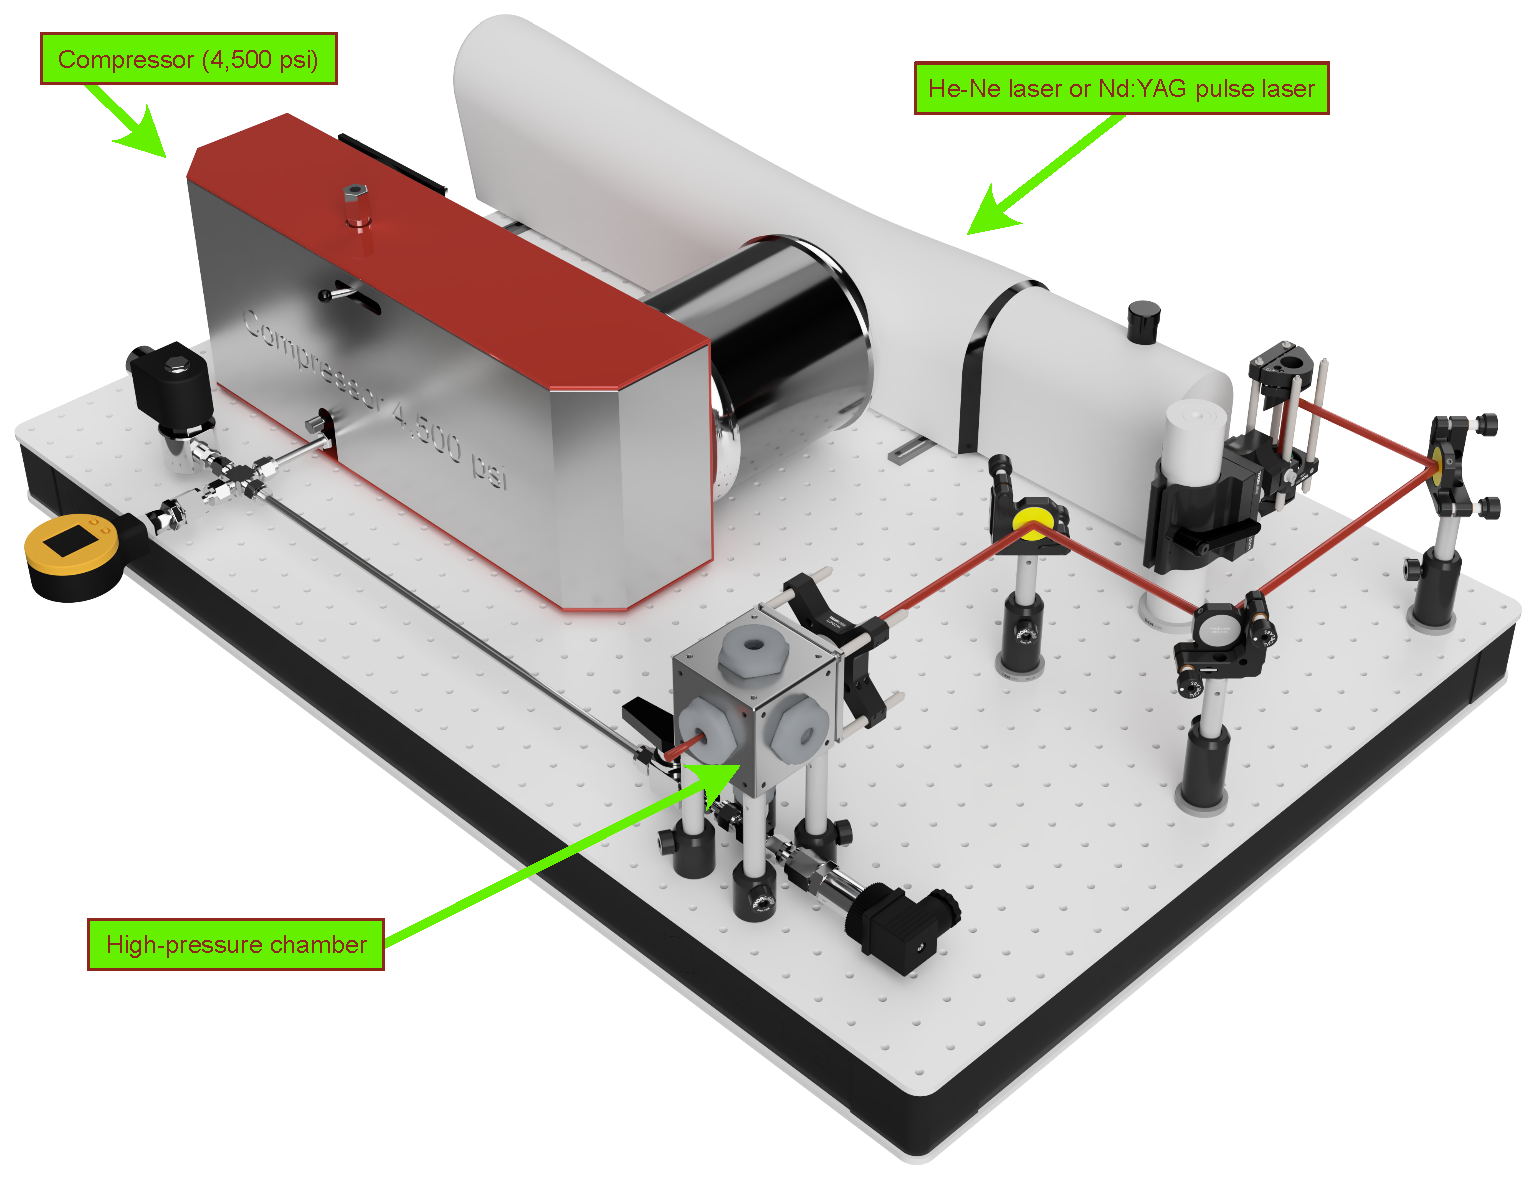
\includegraphics[width=130mm]{figures/ch2/setup/render.pdf}
\caption{Rendered image of experimental apparatus. A cube-shaped high-pressure chamber is located at the bottom of the middle of the image. In the image, Nd:YAG laser is placed, but an additional He-Ne laser is adopted in the same optical path for the diagnostic purpose. The three right-angle viewports are used to take a scattering image of droplets or interferograms. The same setup is utilized to generate laser produced plasma in the supercritical fluid which will be discussed in Chap.\ref{sec:ch4}. The images of plasma and light emission from plasma are also captured through side viewports. All the parts of the system are suitably selected to sustain the designed pressure safely and reliably.}
\label{fig:render}
\end{figure}

\begin{figure}[t!]
\centering
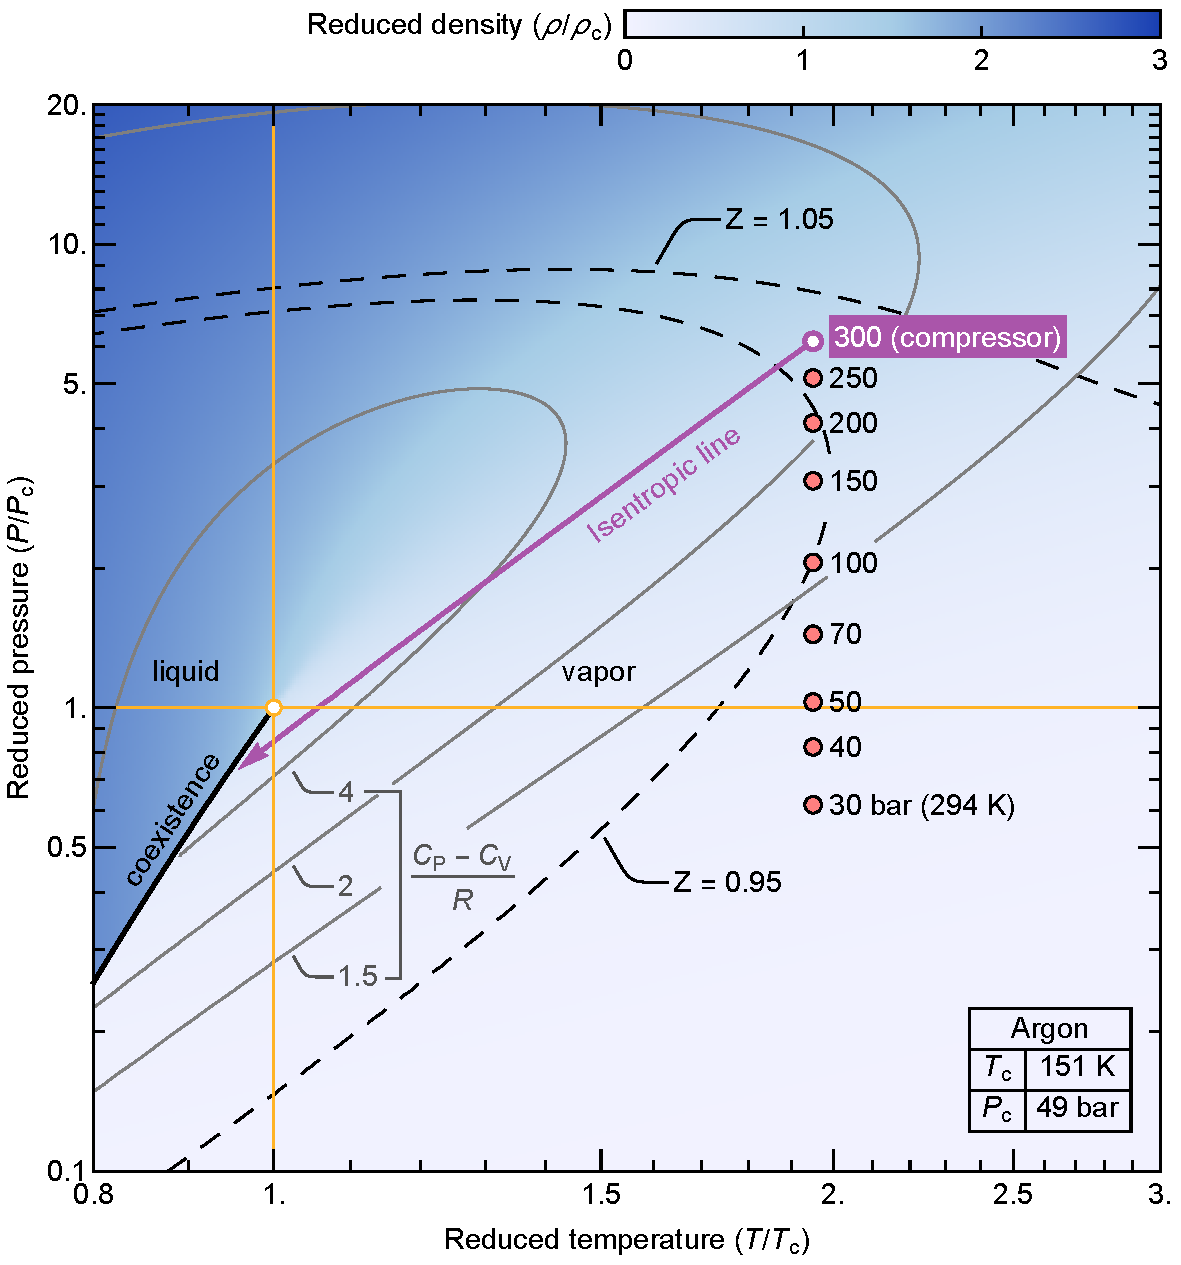
\includegraphics[width=100mm]{figures/ch2/phaseDiag/phaseDiag.pdf}
\caption{Extended phase diagram of homogeneous and equilibrium argon fluid. The red points on the graph represent the experimental conditions. The compressor has a working pressure of $300 \text{ bar}$. The argon fluid undergoes an adiabatic expansion to form the liquid droplets and clusters. The compressibility factor, which writes $Z=P/ρRT$, is unity for the case of an ideal gas. The NIST Chemistry WebBook provides information on argon's thermophysical characteristics \cite{linstorm2020nist}.}
\label{fig:phaseDiag}
\end{figure}

\begin{figure}[t!]
\centering
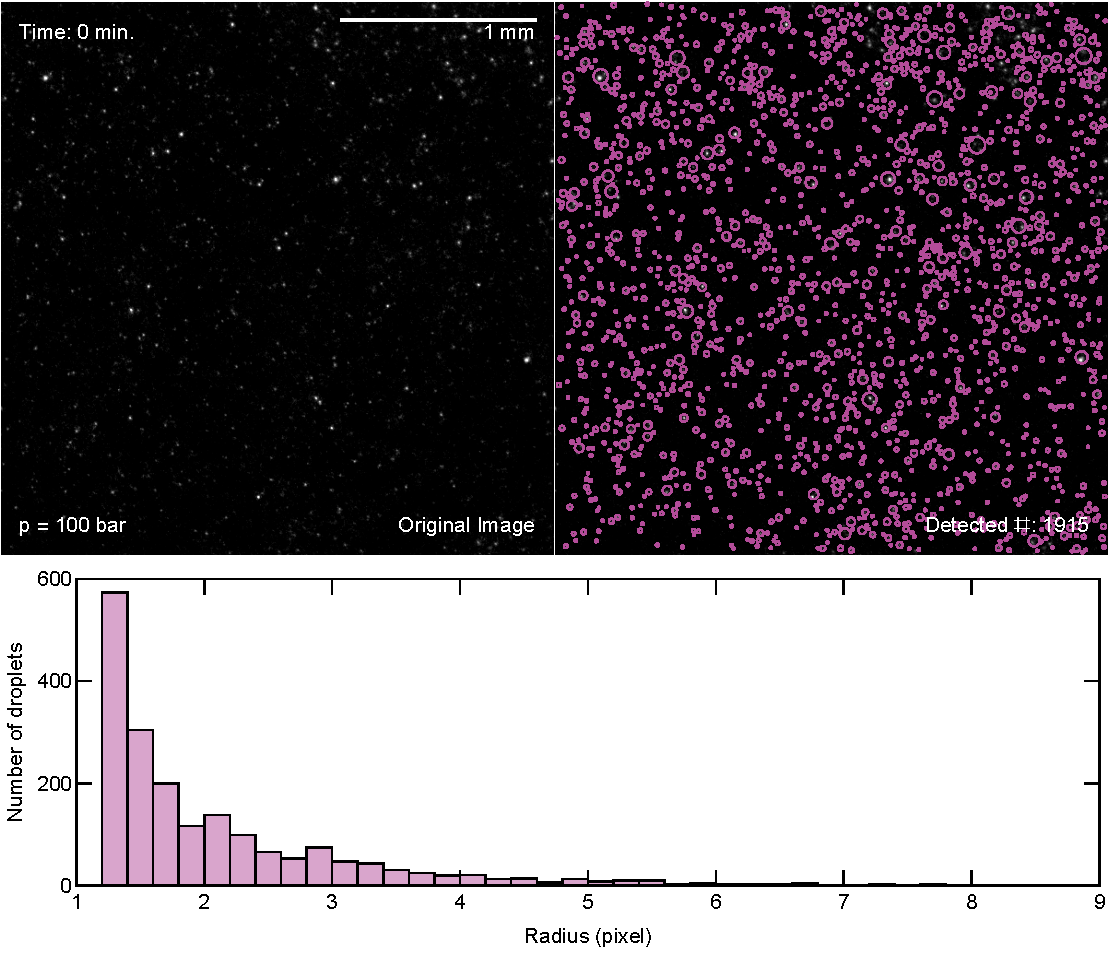
\includegraphics[width=130mm]{figures/ch2/droplet/imgProcess.pdf}
\caption{Image of the scattering signal from droplets with 2.5X magnification and their number counting. The image processing code for counting the number of droplets is not perfect but still reasonably perform. Note that 1 pixel corresponds to $4.8 ~\mathrm{\mu}\text{m}$, but the size measured in this image does not provide the actual size of the droplet due to the diffraction limit.}
\label{fig:imgProcess}
\end{figure}

A check valve (opening pressure: 300 bar) allows argon fluid to enter the high-pressure chamber from a reciprocating compressor. The compressor delivers roughly $6.8\text{ cm}^3$ of argon fluid per cycle (under the standard condition). The extended phase diagram of supercritical argon in Fig.\ref{fig:phaseDiag} \cite{linstorm2020nist, banuti2017similarity} shows a series of experiments along the line of red dots. Because the temperature is around two times above the critical temperature, spontaneous critical phenomena such as density fluctuations do not occur; yet, during compression, the fluid expands rapidly and adiabatically cools to form a liquid. When the argon fluid cools below 140 K, it experiences a phase transition, resulting in the formation of liquid droplets and clusters. The temperature drop of an expanding fluid is well understood (see \cite{hagena1981nucleation, chen2009pressure, tao2016revisiting}), and in Chap.\ref{sec:ch2-3-1}, we compare our experimental results to the COMSOL Multiphysics simulations.

The imaging optics with the ICCD camera captures images and videos of droplets with two different magnifications (2.5X and 11X). The droplets are individually identified owing to their higher Rayleigh–Mie scattering intensity compared to the scattering intensity of the argon fluid and clusters in the background \ref{fig:imgProcess}. The number density and the mean size of droplets are obtained from the lower- and higher-magnification data, respectively. For the lower magnification, the incident He-Ne laser is modified to a beam sheet with a laser line generator (or Powell lens) having the thickness of $100 ~\mu\text{m}$, which is used to calculate the volume number density of droplets from the 2D imaging result. Note that the size of individual droplets cannot be measured by direct imaging because of the diffraction limit of the visible light (light source: 633 nm He–Ne laser). Hence, Brownian motion analysis is adopted to determine the mean size of the droplets.



%----------------------------------------------------------------------------------------------------
\section{Formation of droplets and clusters}
\label{sec:ch2-3}

%----------
\subsection{Temperature drop of expanding fluids}
\label{sec:ch2-3-1}

We perform fluid/heat transport models (using the multiphysics modeling tool COMSOL) and compare them to the results to show that the expanding argon fluid achieves a low enough temperature to become a liquid. A thermocouple with a finite heat capacitance may not experience noticeable cooling since the compressor only delivers a tiny amount of fluid per cycle. As a result, we devised a temperature measurement system that involved filling a small buffer chamber with 300 bar of argon fluid and then abruptly purging it to record the temperature reduction using a thermocouple. The experimental data for the temperature profile along the axis are shown in Fig.\ref{fig:comsolSolenoid}, along with a comparison to simulations. The thermocouple is set $20-60 \text{ mm}$ away from the valve exit in the experiment. To compare with the experiment, each simulation result is averaged spatially inside the red dashed area and temporarily for $0-200 \text{ ms}$.

\begin{figure}[t!]
\centering
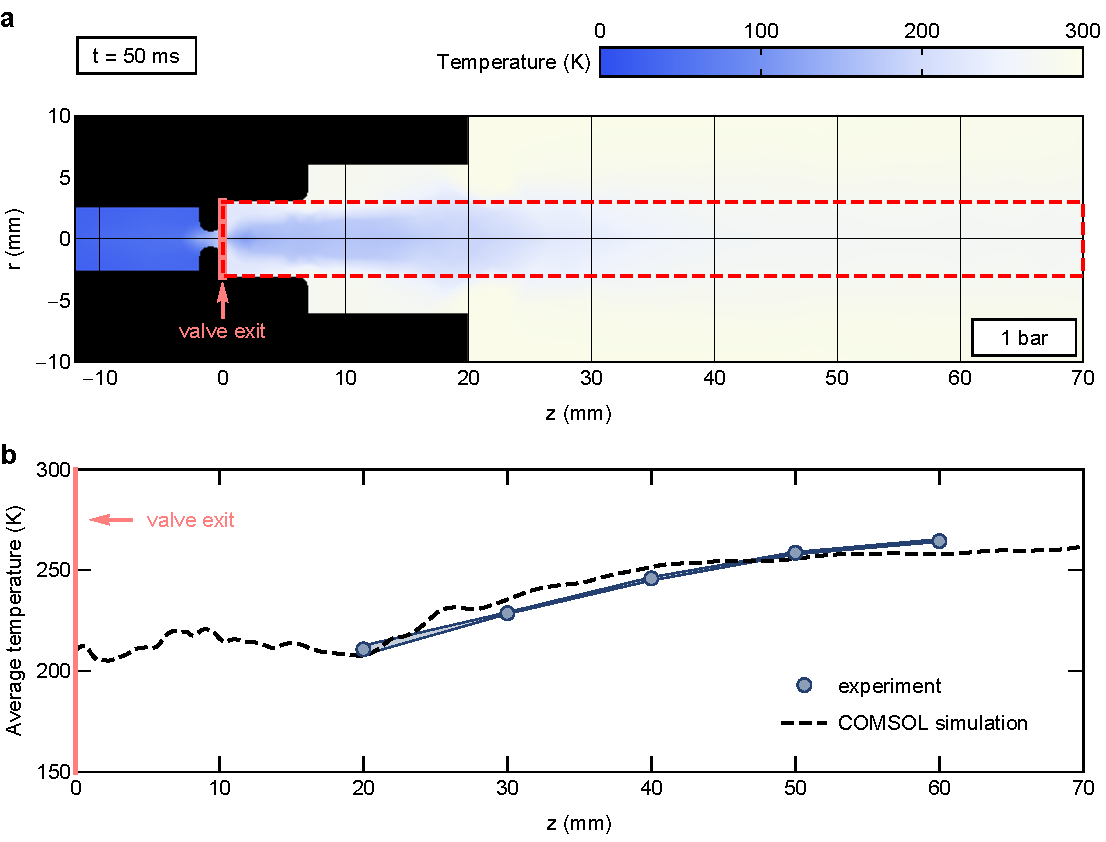
\includegraphics[width=130mm]{figures/ch2/comsol/comsolSolenoid.pdf}
\caption{A temperature drop of an expanding fluid through the solenoid valve from a buffer chamber and comparing the experimental results with the COMSOL Multiphysics simulations. The argon fluid of $300 \text {bar}$ filled in the buffer chamber suddenly expands into the air through the solenoid valve, and the thermocouple monitors the minimum temperature reached. \textbf{a,} The buffer chamber with 300 bar suddenly expands to an open space having 1 bar. \textbf{b,} The experimental measurement is compared with the time- and space-averaged temperature in the simulation results (0-200 ms, red dashed area). The error bands are the standard deviations of each point.}
\label{fig:comsolSolenoid}
\end{figure}

\begin{figure}[t!]
\centering
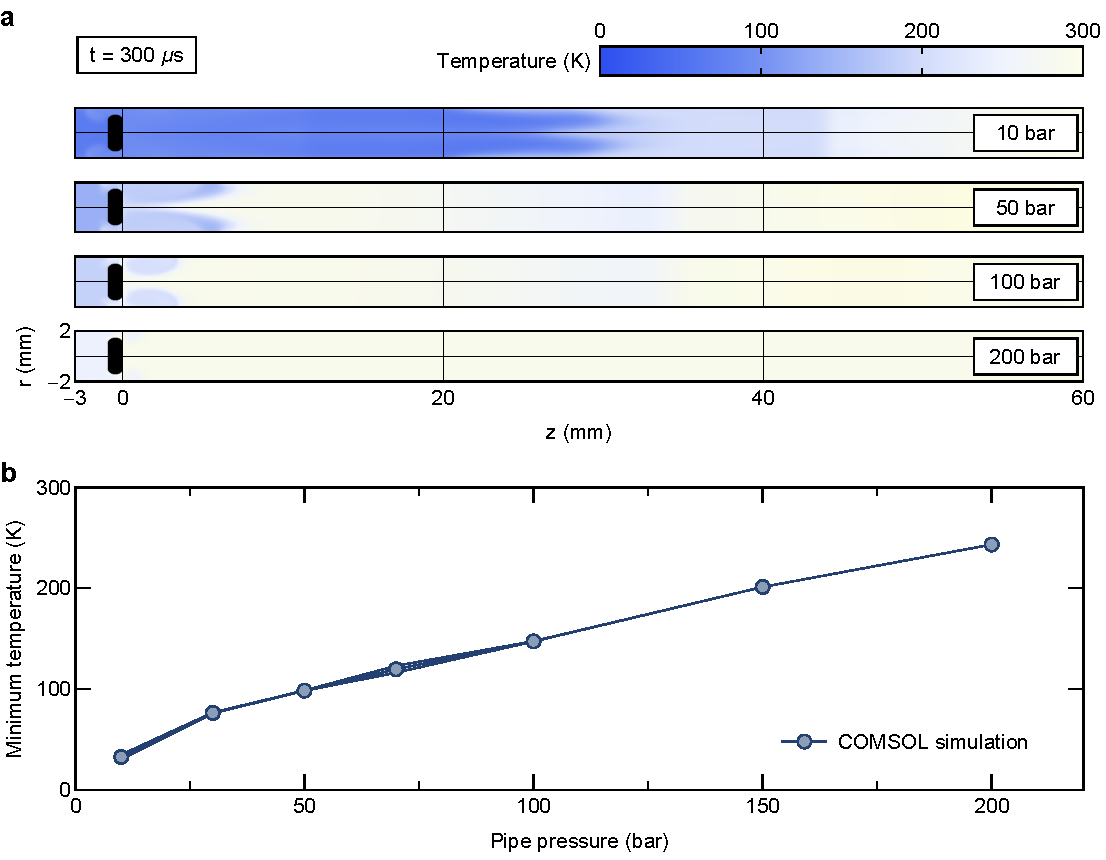
\includegraphics[width=130mm]{figures/ch2/comsol/comsolCompressor.pdf}
\caption{A temperature drop of an expanding fluid through the check valve of the compressor by COMSOL Multiphysics simulations. \textbf{a,} A set of simulations shows the fluid expansion through the check valve of the compressor outlet to the pipe connecting to the main chamber as a function of the initial pipe pressure. \textbf{b,} Minimum temperatures for different pipe pressures. The error bands are the standard deviations of each point.}
\label{fig:comsolCompressor}
\end{figure}

Another set of simulations depicts the temperature profile as the fluid expands abruptly through the compressor's check valve and then into the pipe connecting the main chamber (Fig.\ref{fig:comsolCompressor}). As the original pipe pressure rises, the gradient of the temperature profile reduces. For instance, Fig.\ref{fig:comsolCompressor}b shows the minimum temperature reached within the simulation volume by varying the pipe ($z>0$) pressure. When the pipe pressure is below 100 bar, the fluid cools to the point where it can form a liquid, which corresponds to the creation of droplets and clusters shown in Fig.\ref{fig:numdens}a and Fig.\ref{fig:opacity}a.

Because of heat conduction at the pipe surface, the overall temperature inside the chamber remains unaltered from ambient temperature despite the low local fluid temperature. Using the simplified dimensions of the stainless steel pipe ($r∼2 \text{ mm}$, $l∼800 \text{ mm}$, and $d∼10 \text{ mm}$, where $r$, $l$, and $d$ are the inner diameter, the total length, and the thickness of the pipe, respectively) and the thermal conductivity of a stainless steel $k \sim 16 \text{ W m}^{-1}\text{K}^{-1}$ and assuming the temperature difference between the inside and outside of the pipe $\delta T \sim 10 \text{ K}$, the heat transfer rate becomes
\begin{equation}
\frac{d Q}{d t} \sim k \left( \frac{2 \pi r l}{d} \right) \delta T \sim 160 \text{ W}
\end{equation}
In the experiment, the compressor delivers $N_1 \sim 2.7 \times 10^{-4} \text{ mol} \cdot \text{cycle}^{-1}$, and operates in $f \sim 4.1 \text{ Hz}$. Thus, the number of particles compressed into the chamber per unit time is $N = N_1 \cdot f \sim 1.1 \times 10^{-3} \text{ mol} \cdot \text{s}^{-1}$. Considering the power required to raise the temperature of such fluid from $100$ to $300 \text{ K}$,
\begin{equation}
P_{\text {heat}}=\bar{C}_{\text{P}} N \Delta T \sim 5.5 \text{ W}
\end{equation}
where the average heat capacitance $\bar{C}_{\text{P}} \sim 25 \text{ J K mol}^{-1}$ within the given temperature range under $10 \text{ bar}$ \cite{linstorm2020nist}. The conductive heat transfer rate through the pipe is much faster than the heating power, allowing the chamber to maintain a constant temperature. In the COMSOL simulation, this conclusion is also validated. Further compression to higher pressure increases convective heat transport, which helps keep the temperature of the fluid in the chamber.

%----------
\subsection{Number density of droplets}
\label{sec:ch2-3-2}

\begin{figure}[ht!]
\centering
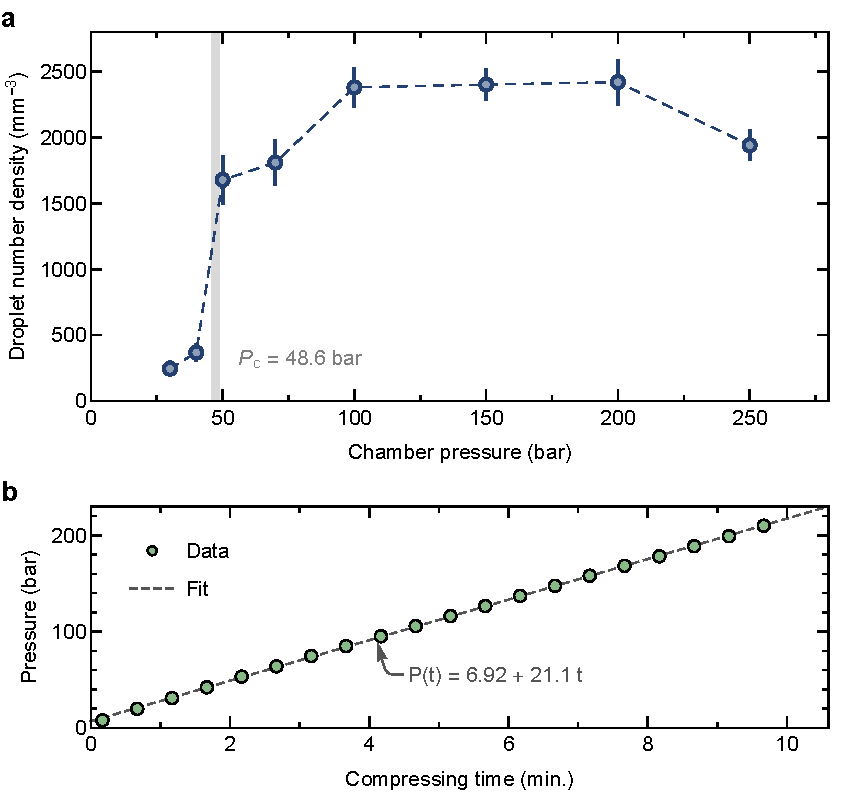
\includegraphics[width=100mm]{figures/ch2/droplet/numdens.pdf}
\caption{Production of droplets. \textbf{a,} The number density of droplets generated by the continual compression of argon fluid in the high-pressure chamber. The droplet number density does not increase as the pressure exceeds $100 \text{ bar}$ because the temperature drop is not large enough to form a liquid at a higher chamber pressure (i.e., a smaller pressure difference between the chamber and check valve) and the droplets evaporate. The number density of droplets decreases due to evaporation in the medium. \textbf{b,} The compression rate by time. There is a competition between the generation and evaporation of droplets, as a finite time is required to raise the chamber pressure.}
\label{fig:numdens}
\end{figure}

In terms of droplet density, average lifetime of droplets, and medium opacity, Fig.\ref{fig:numdens}, \ref{fig:lifetime}, and \ref{fig:opacity} shows how SCF properties change as pressure increases. The substantial changes in these properties across the critical pressure are worth noting. The abrupt increase in droplet density over the critical pressure, above which it is saturated, is depicted in Fig.\ref{fig:numdens}a. Through the check valve, argon gas is cumulatively compressed into the chamber, forming liquid droplets and clusters. As the chamber pressure rises, the droplet creation rate falls, and droplet formation eventually ceases. It is consistent with the COMSOL simulation results – a sufficient temperature drop to form a liquid during a sudden expansion occurs when the chamber pressure is below $100 \text{ bar}$ (Fig.\ref{fig:comsolCompressor}b). The droplets formed during compression evaporate within the fluid as well. The number density of droplets does not keep increasing throughout the compression, as shown in Fig.\ref{fig:numdens}a. Instead, the generation and evaporation of the droplets co-occur and compete, and finally, above $100 \text{ bar}$, evaporation dominates.

%----------
\subsection{Lifetime of droplets}
\label{sec:ch2-3-3}

\begin{figure}[ht!]
\centering
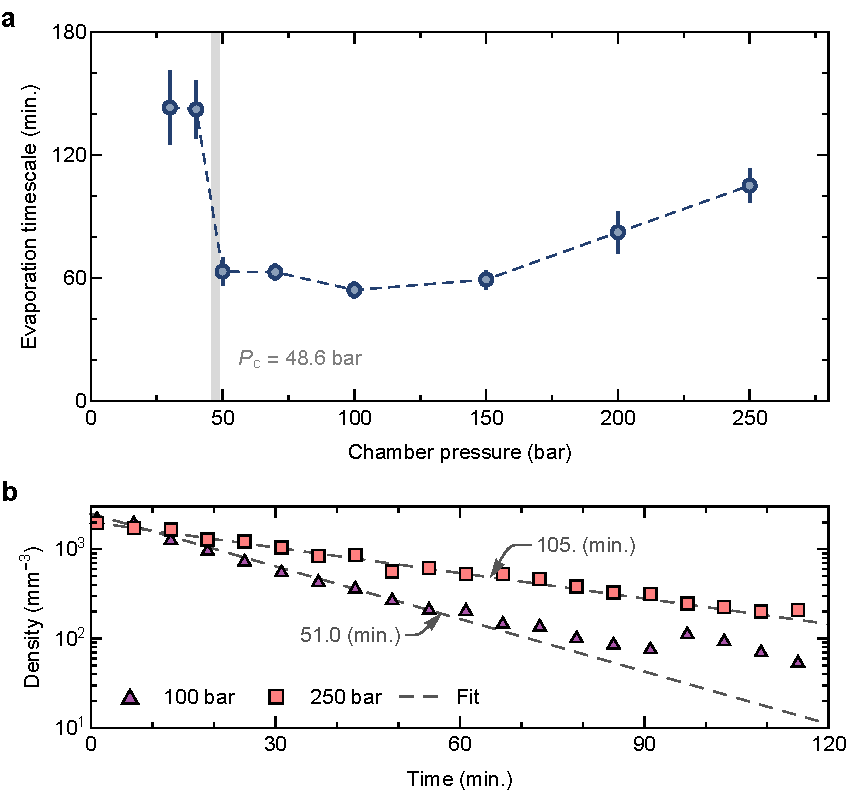
\includegraphics[width=100mm]{figures/ch2/droplet/evaporation.pdf}
\caption{Lifetime of droplets. \textbf{a,} The evaporation timescale of the droplets at different pressures. The evaporation timescale of LL droplets exceeds two hours below the critical pressure and suddenly decreases to an hour above the critical pressure. Again, the evaporation timescale is extended with increasing pressure above the critical pressure. \textbf{b,} Exponential decrease of the droplet's number density. The number density of the droplets decreases as time goes, and the characteristic lifetime is defined when the density reaches below $1/10$th of the initial value.}
\label{fig:lifetime}
\end{figure}

At varied chamber pressures, the lifetime of droplets or the evaporation timescale (defined by the period when the droplet number density becomes $1/10\text{th}$ of the maximum) is illustrated in Fig.\ref{fig:lifetime}a. The droplet number density is monitored for two hours after compression for each pressure condition. The evaporation timeframe decreases and eventually increases when the chamber pressure is increased above the critical pressure. We use the evaporation model and the consequent cluster effect to explain both the abrupt change at the critical pressure and the monotonic ascent at higher pressures in Chap.\ref{sec:ch2-5}.

%----------
\subsection{Existence of clusters}
\label{sec:ch2-3-4}

\begin{figure}[ht!]
\centering
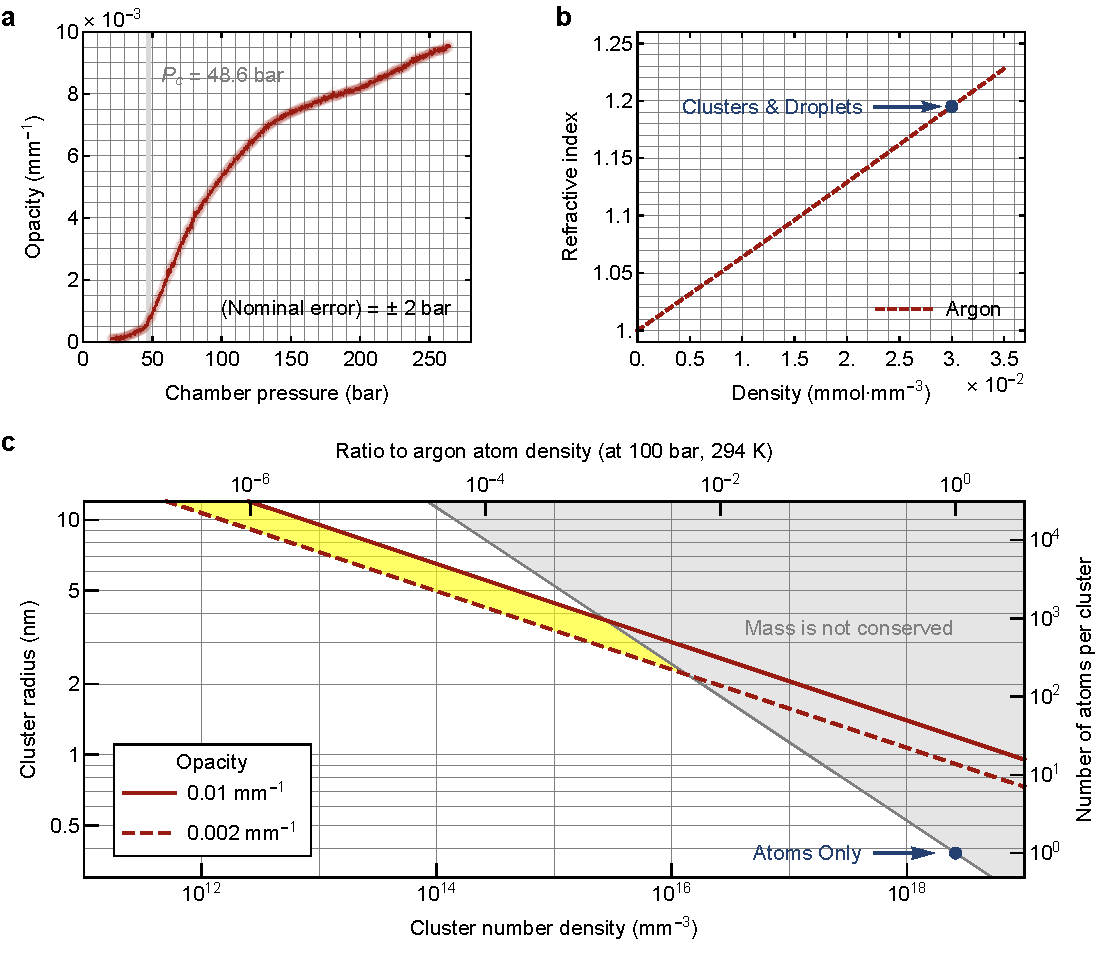
\includegraphics[width=130mm]{figures/ch2/cluster/opacity.pdf}
\caption{Opacity analysis for the existence of the nanometer-sized clusters. \textbf{a,} Opacity of the high-pressure chamber while compressing. It is not sufficient to obtain such opacity with the droplets only. \textbf{b,} Refractive index for the LL clusters and droplets. The refractive index for LL argon fluid packages is assumed to be that of the liquid argon at about $100 \text{ K}$. \textbf{c,} Expected number density and size of the clusters to satisfy the opacity measurement. The gray shaded area is forbidden because the number of atoms exceeds the total number of atoms for the given chamber conditions ($100 \text{ bar}$, $294 \text{ K}$). The clusters should have density and size within the yellow shaded area. The dark-blue dot corresponds to the opacity for the case of atoms only (i.e., no clusters).}
\label{fig:opacity}
\end{figure}

The opacity inside the chamber rapidly increases, such as in Fig.\ref{fig:opacity}, which we attribute to the formation of a significant number of clusters. It is worth noting that these clusters are created by a compression-expansion process rather than by critical phenomena.

Clusters, unlike drops, are too tiny to be distinguished separately. They increase the medium opacity through the Rayleigh scattering and absorption. To ensure that these clusters, not the droplets, are responsible for the majority of the opacity, we calculate the opacity due to particle scattering as follows:
\begin{equation}
\chi \left( \lambda \right) = \sum_{\text{s}} n_{\text{s}} \sigma_{\text{s}} \left( \lambda \right)
\end{equation}
where $n_\text{s}$ and $\sigma_\text{s}$ are the number density and the total scattering cross-section of the particle species s (droplets, clusters, and atoms), respectively \cite{fivsak2016rayleigh, hulst1981light, howell2020thermal}, and $\lambda$ is the wavelength of the incident light. For a large particle with a size comparable to $\lambda$, $\sigma \sim \pi r^2$ where $r$ is the mean radius of the particles. The upper limit of the opacity caused by the droplets is about $0.002 \text{ mm}^{-1}$ (using $n_\text{d} \sim 2500 \text{ mm}^{-3}$ around $150 \text{ bar}$ and $r_\text{d} \sim 0.5 \times 10^{-3} \text{ mm}$, see Fig.\ref{fig:numdens} and \ref{fig:size}), which is quite small, implying that the major contribution to opacity comes from the clusters and not from the droplets.

The Rayleigh scattering cross-section of a small particle with radius $r$ is
\begin{equation}
\sigma = \frac{2 \pi}{3} \frac{\left( 2 r \right)^{6}}{\lambda^{4}}\left( \frac{n^{2}-1}{n^{2}+2} \right)^{2}
\end{equation}
where $\lambda$ is the wavelength of the incident light and n is the refractive index ratio between the particle and a medium \cite{howell2020thermal}. The criteria of cluster size and number density required to attain such opacity are shown in Fig.\ref{fig:opacity}c. The gray area is  where the mass conversation is violated for the given condition ($100 \text{ bar}$, $294 \text{ K}$). A cluster is assumed to have $n \sim 1.2$ – the value for a liquid argon at about $100 \text{ K}$ \cite{hanna2010equation}. To explain the measured opacity, the cluster conditions should be in the yellow highlighted area. The chamber opacity for the situation of ``atoms only'' is nowhere near the experimental result (note the dark-blue point in Fig.\ref{fig:opacity}). As a result, the clusters are the primary cause of the medium's fogginess and opacity.

As we will see later, a large number of clusters in the argon fluid have a significant impact on mass transfer at the droplet surface. In addition, the evaporation timescale of the droplets is affected by the clusters in the SCF.


%----------------------------------------------------------------------------------------------------
\section{Brownian motion analysis}
\label{sec:ch2-4}

%----------
\subsection{Droplet size}
\label{sec:ch2-4-1}

\begin{figure}[ht!]
\centering
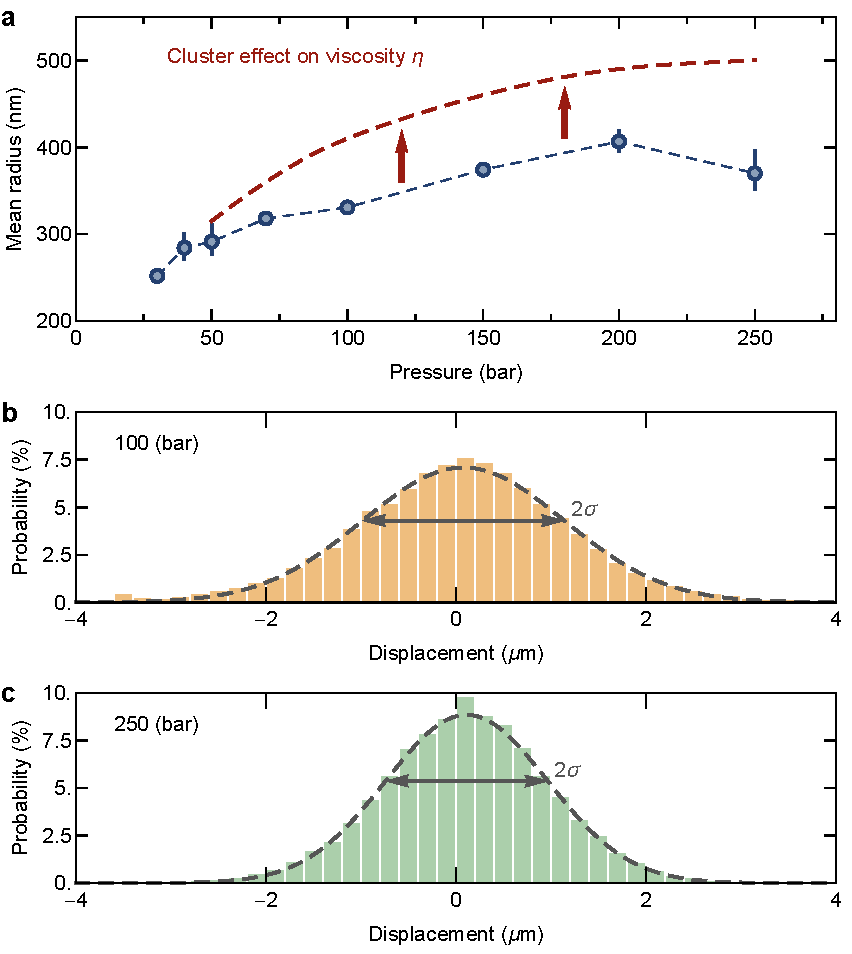
\includegraphics[width=100mm]{figures/ch2/Brownian/size.pdf}
\caption{Mean size of droplets at different pressures. \textbf{a,} The mean size at each pressure is calculated using Brownian motion analysis. The motions of the droplets are divided into two axes, yielding two sets of one-dimensional displacements. With the emergence of the clusters, the medium viscosity tends to decrease. The green dashed line shows the difference in anticipated droplet sizes when the cluster effect on viscosity is taken into consideration in a condition with a high cluster density, as in our experiments. The error band shows $90\%$ confidence interval of normal distribution fit for each pressure. \textbf{b-c,} The histograms show the displacement of droplets during the elapsed time ($0.02 \text{ s}$) and their normal distribution fits at $100 \text{ bar}$ and $250 \text{ bar}$, respectively.}
\label{fig:size}
\end{figure}

Visual inspection of the argon SCFs reveals a large number of submicron-sized droplets. The droplets, in particular, persist for a long time, allowing us to measure the size using direct imaging and Brownian motion analysis.

Brownian particles floating in argon fluid are used to calculate the average size of droplets. High-resolution imaging optics (11X magnification) and ICCD track the small displacements of droplets caused by their jiggling motion (50 frames per second). The videos are taken three minutes after compression, allowing any turbulence in the medium to be stabilized at each operating pressure. 

The mean squared displacement $\sigma^2$ of Brownian particles for one-dimensional motion is expressed by the following equation \cite{einstein1956investigations}:
\begin{equation}
\sigma^2 = 2Dt
\end{equation}
where $D$ is the diffusion coefficient of the surrounding medium and t is the elapsed time (in our experiment, $t=0.02 \text{ s}$). The Stokes-Einstein equation relates the diffusion coefficient to the mean radius $r$ of the Brownian particles \cite{einstein1956investigations}:
\begin{equation}
D=\frac{k_\text{B} T}{6\pi \eta r}
\label{eq:einstein}
\end{equation}
where $k_\text{B}$, $T$, and $\eta$ are the Boltzmann constant, the temperature, and the dynamic viscosity of the surrounding medium, respectively. We referred to the NIST Chemistry WebBook \cite{linstorm2020nist} for the dynamic viscosity of argon at each pressure. The mean radius of the droplets, based on the dynamic viscosity, varies from about $250$ to $400 \text{ nm}$ depending on the final chamber pressure, as shown in Fig.\ref{fig:size}a. Using a homogeneous medium viscosity, on the other hand, may introduce errors in size estimation if the medium contains a large number of clusters. This is because when some portions of the medium are clustered, the viscosity is lower than when the medium is homogeneous, resulting in underestimating the droplet size. In Chap.\ref{sec:ch2-4-2}, we will go over this in more detail.

%----------
\subsection{Viscosity correction for a clustered medium}
\label{sec:ch2-4-2}

The size estimation by the Brownian motion analysis obtained through Eq.\ref{eq:einstein} depends on the accuracy of the medium viscosity. We used the viscosity value for a homogeneous argon fluid at the given pressure and temperature from the NIST Chemistry WebBook \cite{linstorm2020nist} in our calculations. However, as the pressure rises, more clusters form in the medium, and it is crucial to understand how this affects the fluid's viscosity. Therefore, instead of a comprehensive viscosity analysis, a simplified analysis will suffice to show that the viscosity of the clustered medium will be lower than that of the homogeneous medium.

According to the kinetic model, the viscosity $\eta$ of a medium consisting of spherical particles of radius $r$ and mass $m$ is
\begin{equation}
\eta \propto \frac{\sqrt{m T}}{\pi r^{2}}
\end{equation}
where $T$ is the temperature of the medium \cite{chapman1990mathematical}. The proportionality constant may be temperature dependent when considering particle interaction, but the fundamental relationship does not change significantly. Assume that each cluster has an average of $N$ argon atoms and that the temperature is constant, the proportionality of the viscosity writes
\begin{equation}
\eta \propto N^{-1 / 6}
\end{equation}
as $m \propto N$ and $r \propto N^{1/3}$. As a result, if atoms aggregate to form clusters, the viscosity of the medium decreases, and the droplet size is underestimated for a higher cluster density. The green dashed curve in Fig.\ref{fig:size} illustrates the cluster effect on droplet size estimation.

In conclusion, we show that droplets can survive for long periods in SCF. However, according to the analysis of mass transport, the clustering effect can reduce the lifetime of droplets, implying that the clustering effect is crucial to understanding non-equilibrium thermodynamic processes in supercritical states.

The existence of quasi-steady clusters and droplets will have practical implications in planetary meteorology, power plant cooling systems, pharmaceutical processes, high-power switching, and high-pressure fuel injection, among other fields of science and engineering involving SCFs. Clusters and droplets, for example, may have an impact on mass transport processes in Venus' and Jupiter's dense atmospheres. In the recent development of the SCF CO2 cleaning technique in semiconductor fabrication, the same effect may have to be considered. Our findings are expected to be a turning point in studying SCFs' non-equilibrium, transient behavior. The physics that supports clusters and droplets in SCFs will be a widespread issue in various engineering problems involving heat and momentum transport processes in SCFs.

%----------
\subsection{Size distribution}
\label{sec:ch2-4-3}

The Brownian motion analysis provides the size of the droplets, and we might be wondering how the calculation will be affected if the size distribution changes. For the brief answer, this analysis gives the average of any size distribution. That is to say, with this statistical analysis, the distribution information is screened, and only the average of particular size distribution remains. Thus, technically, the radius from Eq.\ref{eq:einstein} represents the `arithmetic mean' of the size distribution.

\begin{figure}[ht!]
\centering
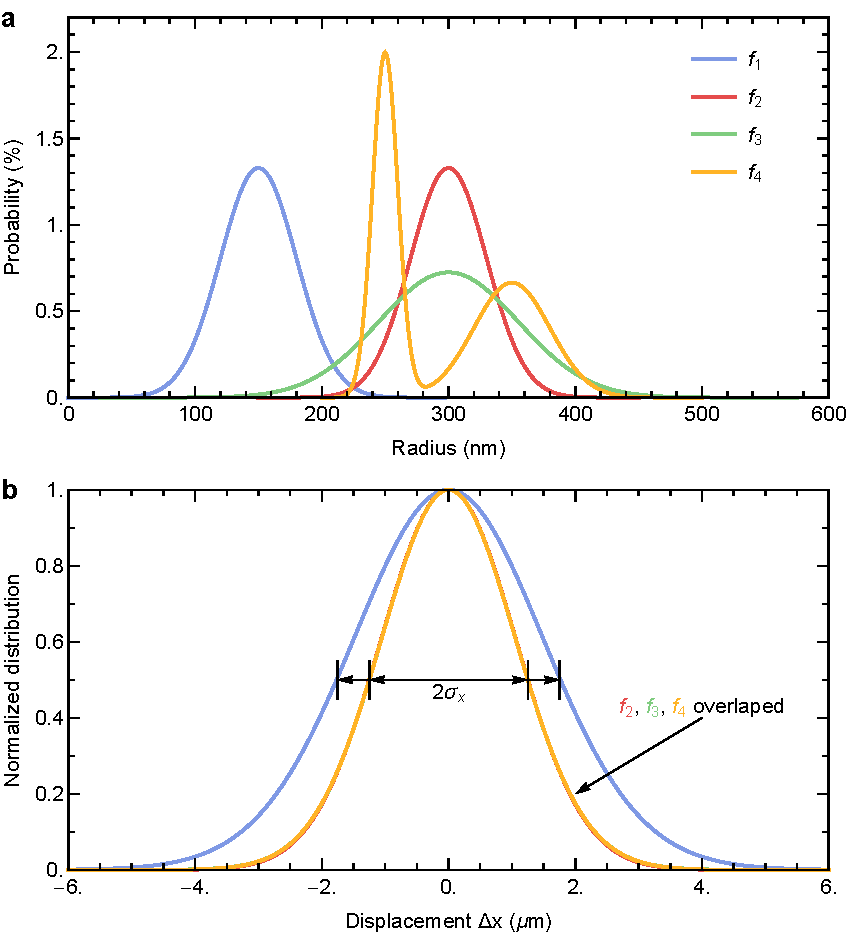
\includegraphics[width=100mm]{figures/ch2/Brownian/distributionEffect.pdf}
\caption{Four different artificially designed distribution functions and their resulting particle displacements distributions. \textbf{a,} The functions follow the normal distributions with different parameters ($f_1$, $f_2$, and $f_3$), or combination of two normal distributions ($f_4$). The mean of function $f_4$ is set to be the same with that of functions $f_2$ and $f_3$ \text{b,} The resulting displacements distributions from each size distributions. The physical values -- $T=294 \text{ K}$ and $\eta \sim 2.53\times10^{-5} \text{ Pa}\cdot\text{s}$ are used to append the units of the order of the experimental results.}
\label{fig:distributionEffect}
\end{figure}

\begin{table}[h!]
\footnotesize
\centering
\begin{tabular}{c|cccc}
                    & $f_1$   & $f_2$   & $f_3$  & $f_4$   \\ \hline
$m_r$          & 150     & 300    & 300    & 300 \\
$\sigma_r$   & 30.0    & 30.0    & 55.1    & 54.8 \\
$\sigma_x$  & 2.28    & 1.14    & 1.14    & 1.14
\end{tabular}
\caption{Statistical information of distribution functions. The four functions have the different mean size $m_r$, the standard deviation of size $\sigma_r$, and the resulting standard deviation of displacements of Brownian particles $\sigma_x$. The standard deviations of displacements follow the mean size and are not affected by the shape of the original distribution function.}
\label{table:standardDeviation}
\end{table}

To check how the size distribution of particles contributes to the Brownian motion analysis, we introduce four artificially designed distribution functions having different means and standard deviations (Fig.\ref{fig:distributionEffect}a):
\begingroup
\allowdisplaybreaks
\begin{align}
f_1 &= C_1 e^{ - \frac{1}{2} \left( \frac{r - 150}{30} \right)^2 } \\
f_2 &= C_2 e^{ - \frac{1}{2} \left( \frac{r - 300}{30} \right)^2 } \\
f_3 &= C_3 e^{ - \frac{1}{2} \left( \frac{r - 300}{55} \right)^2 } \\
f_4 &= C_4 \left[ e^{ - \frac{1}{2} \left( \frac{r - 250}{10} \right)^2 } + e^{ - \frac{1}{2} \left( \frac{r - 350}{30} \right)^2 } \right]
\end{align}
\endgroup
, where $C_1$ through $C_4$ are the normalization factors. For each size distribution, the displacement distribution is retrieved (Fig.\ref{fig:distributionEffect}b). In other words, the displacements of virtual particles where the population distribution follows the given functional form are calculated. As in the Table. The standard deviation of the displacements of virtual Brownian particles is decided by the mean of the original distribution function and is not affected by the original function's shape. This shows that the Brownian motion analysis only gives the mean size of the particles and tells nothing about the size distribution.



%----------------------------------------------------------------------------------------------------
\section{Modified evaporation model}
\label{sec:ch2-5}

The estimated droplet radii trend around the critical pressure (Fig.\ref{fig:size}a) appears to conflict with the droplet lifetime (evaporation timescale) trend (Fig.\ref{fig:lifetime}a). Thus, smaller droplets below the critical pressure may take longer to evaporate than larger droplets above the critical pressure, based on the two trends. Consider the effect of clusters on mass transport at the droplet surface to resolve this apparent contradiction.

\begin{figure}[t!]
\centering
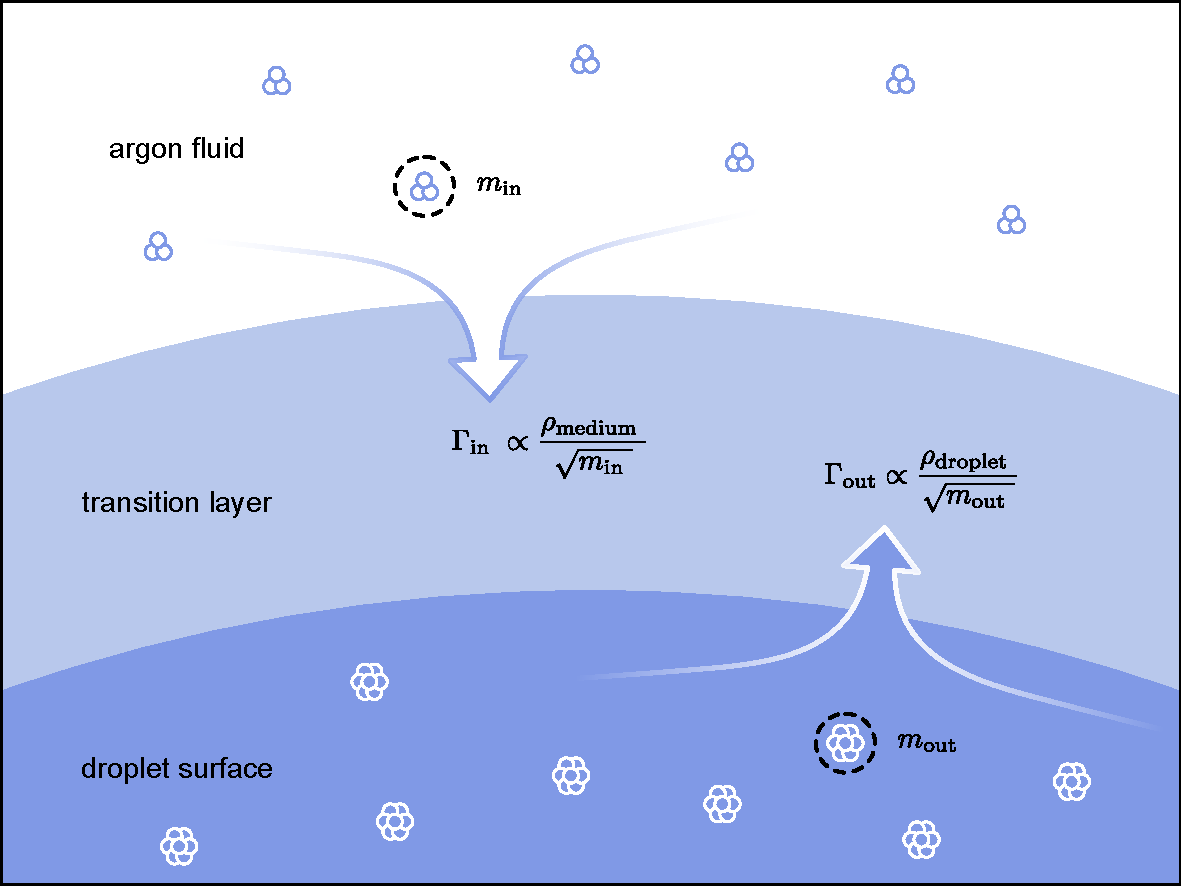
\includegraphics[width=100mm]{figures/ch2/transport/evaporation.pdf}
\caption{Graphical illustration of the mass transport at a droplet surface. The emergence of clusters reduces the mass influx, and consequently, the evaporation time of a droplet decreases. The mass carriers of the influx and outflux are assumed to be clustered, altering the number of particles within a given time interval to be transferred into- or out of- the transition layer.}
\label{fig:evaporation}
\end{figure}

It is impractical to consider all of the interactions between the atoms in a submicron-sized droplet in a dense background fluid to calculate the evaporation timescale. On the other hand, a submicron-sized droplet is large enough to consider evaporation as a surface process. To explain our experimental results, we use an evaporation model similar to that of subcritical fluids \cite{ishiyama2004molecular, julin2013mass}.

The droplet and the surrounding fluid are in a quasi-thermal equilibrium over an hour, implying that mass influx $\Gamma_\text{in}$ would balance mass outflux $\Gamma_\text{out}$ in the transition layer around the droplet surface (illustrated in Fig.\ref{fig:evaporation}), and suggesting that the net mass flux $\Gamma_\text{net}$ is negligible:
\begin{equation}
\begin{aligned}
\Gamma_{\text{net}} &= \Gamma_{\text{out}} - \Gamma_{\text{in}} \\
&= v_{\text{out }} \rho_{\text{out}} - v_{\text{in }} \rho_{\text{in}} \approx 0
\end{aligned}
\end{equation}
where $v_\text{in(out)}$  and $\rho_\text{in(out)}$ are the surface-normal mean velocities and mass densities, respectively. The outflux is defined as the flux leaving the inner boundary of the transition layer, i.e., the surface of the droplet. The surface-normal mean velocity is then
\begin{equation}
v_{\text {in }(\mathrm{out})}=\sqrt{\frac{8 k_{\mathrm{B}} T}{\pi m_{\mathrm{in}(\mathrm{out})}}}
\end{equation}
where $m_\text{in(out)}$ denotes the mass of the mass carrier. Assuming that the droplet has the density of liquid argon  ($\rho_\text{out} = \rho_\text{droplet} = \rho_\text{liquid}$), the net mass flux becomes
\begin{equation}
\Gamma_{\mathrm{net}} \approx \sqrt{\frac{8 k_{\mathrm{B}} T}{\pi}}\left(\frac{\rho_{\text {droplet }}}{\sqrt{m_{\text {out }}}}-\frac{\rho_{\text {medium }}}{\sqrt{m_{\text {in }}}}\right)
\end{equation}
where the mass density of influx $\rho_\text{in} = \rho_\text{medium}$. The evaporation timescale would be prolonged if the net flux remained insignificant.

When the critical pressure is crossed, the number of clusters in the medium suddenly rises, as shown in Fig.\ref{fig:opacity}a, and the average mass of the mass carrier of the particle influx $m_\text{in}$ increases. As a result, the influx is lowered substantially, and the evaporation period is shortened (see the region around the critical pressure in Fig.\ref{fig:lifetime}a). On the other hand, the number of clusters is less at subcritical pressures, thus the influx is greater, resulting in a considerably longer evaporation period (the higher pressure condition in Fig.\ref{fig:lifetime}a). If the pressure rises to the point where it surpasses the critical pressure, the number of clusters increases as well. However, as $\rho_\text{medium}$ gradually approaches $\rho_\text{droplet}$, the overall flux is rebalanced, resulting in a prolonged evaporation timescale.
